\section{Module 5: Tự động hóa Khai báo Hạ tầng với OpenStack Heat}

\subsection{Mục tiêu \& Mô hình Hạ tầng dưới dạng Mã (IaC)}
Nếu như ở các Module từ 1 đến 4, nhóm chúng em đã tìm hiểu và làm quen với quy trình quản trị hạ tầng theo từng bước mệnh lệnh thủ công (Imperative Approach), thì trong môi trường doanh nghiệp quy mô lớn, phương pháp này bộc lộ nhiều hạn chế về thời gian triển khai, khó kiểm soát phiên bản và dễ phát sinh sai sót do con người. Để khắc phục triệt để, tại Module 5, nhóm chúng em áp dụng mô hình Hạ tầng dưới dạng Mã (Infrastructure as Code - IaC) thông qua công cụ điều phối \textbf{OpenStack Heat Orchestration Engine}~\cite{heat_hot_guide}.

Bằng phương pháp tiếp cận khai báo (Declarative Approach), toàn bộ kiến trúc hạ tầng phức tạp bao gồm: mạng ảo Neutron, router L3, security group, cổng mạng, địa chỉ Floating IP, ổ đĩa Cinder, máy ảo Nova và kịch bản nạp ứng dụng tự động qua Cloud-Init~\cite{cloudinit_docs} đều được chúng em gói gọn bên trong một tệp mẫu duy nhất mang tên \texttt{module5\_service.yaml}.

\subsection{Cấu trúc Mẫu Điều phối Heat (HOT Architecture)}
Mẫu template được nhóm chúng em xây dựng tuân thủ quy chuẩn phiên bản \nolinkurl{heat_template_version: 2021-04-16}. Khi tiếp nhận bản khai báo này, Heat Engine sẽ tự động phân tích các hàm liên kết nội tại (như \texttt{get\_resource} và \texttt{get\_param}) để xây dựng một Đồ thị có hướng không chu trình (Directed Acyclic Graph - DAG), từ đó tối ưu hóa thứ tự cấp phát song song cho 10 khối tài nguyên liên kết chặt chẽ:

\begin{lstlisting}[language=yaml, basicstyle=\ttfamily\scriptsize, caption={Khai báo tài nguyên trong Heat Template (\texttt{module5\_service.yaml}).}]
heat_template_version: 2021-04-16
description: Complete automated stack with network, storage, VM, and cloud-init.

parameters:
  image: { type: string, default: Fedora-Cloud-Base-37-1.7.x86_64 }
  flavor: { type: string, default: m1.small }
  key_name: { type: string, default: module3-key-pair }
  public_network: { type: string, default: public }

resources:
  m5_dmz_net:
    type: OS::Neutron::Net
    properties: { name: m5-dmz-net }

  m5_dmz_subnet:
    type: OS::Neutron::Subnet
    properties:
      network: { get_resource: m5_dmz_net }
      cidr: 10.50.10.0/24
      dns_nameservers: [8.8.8.8, 1.1.1.1]

  m5_router:
    type: OS::Neutron::Router
    properties:
      external_gateway_info: { network: { get_param: public_network } }

  m5_router_interface:
    type: OS::Neutron::RouterInterface
    properties:
      router: { get_resource: m5_router }
      subnet: { get_resource: m5_dmz_subnet }

  m5_web_sg:
    type: OS::Neutron::SecurityGroup
    properties:
      rules:
        - { protocol: tcp, port_range_min: 22, port_range_max: 22 }
        - { protocol: tcp, port_range_min: 80, port_range_max: 80 }
        - { protocol: icmp }

  m5_web_port:
    type: OS::Neutron::Port
    properties:
      network: { get_resource: m5_dmz_net }
      security_groups: [{ get_resource: m5_web_sg }]

  m5_floating_ip:
    type: OS::Neutron::FloatingIP
    properties:
      floating_network: { get_param: public_network }
      port_id: { get_resource: m5_web_port }

  m5_data_volume:
    type: OS::Cinder::Volume
    properties: { name: m5-data-volume, size: 1 }

  m5_server:
    type: OS::Nova::Server
    properties:
      name: m5-web-server
      image: { get_param: image }
      flavor: { get_param: flavor }
      key_name: { get_param: key_name }
      networks: [{ port: { get_resource: m5_web_port } }]
      user_data_format: RAW
      user_data: |
        #!/bin/bash
        for i in {1..30}; do [ -b /dev/vdb ] && break; sleep 2; done
        blkid /dev/vdb || mkfs.ext4 /dev/vdb
        mkdir -p /mnt/app && mount /dev/vdb /mnt/app
        echo "<h1>Module 5 - Heat Automated Deployment</h1>" > /mnt/app/index.html
        nohup python3 -m http.server 80 --directory /mnt/app > /var/log/m5-http.log 2>&1 &

  m5_volume_attachment:
    type: OS::Cinder::VolumeAttachment
    properties:
      volume_id: { get_resource: m5_data_volume }
      instance_uuid: { get_resource: m5_server }

outputs:
  service_url:
    description: URL to access the deployed web application
    value:
      str_replace:
        template: "http://%ip%"
        params: { "%ip%": { get_attr: [m5_floating_ip, floating_ip_address] } }
\end{lstlisting}

\subsection{Pipeline Tự Cấu hình với Cloud-Init}
Một trong những giải pháp kỹ thuật trọng tâm mà nhóm chúng em thiết kế là kịch bản \texttt{user\_data} nhúng trong template, được hệ thống Cloud-Init thực thi tự động ngay khi máy ảo khởi động:
\begin{enumerate}
    \item \textbf{Vòng lặp Thăm dò Thiết bị (Storage Discovery Loop):} Do tiến trình khởi động của máy ảo diễn ra độc lập với quá trình đính kèm volume của Cinder, chúng em lập trình một vòng lặp kiểm tra trạng thái thiết bị khối \texttt{/dev/vdb} tối đa 30 lần (chu kỳ 2 giây/lần). Cơ chế này loại bỏ hoàn toàn hiện tượng tương tranh (Race Condition), đảm bảo script chỉ tiếp tục khi kernel đã nạp hoàn tất driver \texttt{virtio\_blk}.
    \item \textbf{Định dạng \& Gắn Ổ đĩa có Tính Idempotent:} Để phòng ngừa rủi ro ghi đè dữ liệu khi máy ảo tái khởi động, chúng em sử dụng lệnh \texttt{blkid /dev/vdb} kiểm tra sự tồn tại của superblock. Lệnh định dạng \texttt{mkfs.ext4} chỉ được thực thi nếu ổ đĩa hoàn toàn mới, sau đó volume được gắn an toàn vào thư mục \texttt{/mnt/app}.
    \item \textbf{Tự động Hóa Dịch vụ Web:} Kịch bản tự sinh trang giao diện HTML mẫu và kích hoạt máy chủ HTTP nền bằng Python trên cổng 80, điều hướng toàn bộ log tiến trình vào \texttt{/var/log/m5-http.log} để tiện cho việc giám sát.
\end{enumerate}

\subsection{Triển khai Stack \& Xác thực Tự động}
Trước khi khởi chạy, nhóm chúng em tiến hành kiểm tra tính hợp lệ về mặt cú pháp và logic của template, sau đó kích hoạt quy trình tạo stack thông qua OpenStack CLI:
\begin{lstlisting}[language=bash]
$ openstack orchestration template validate -t service.yaml
$ openstack stack create -t service.yaml module5-stack
\end{lstlisting}

\begin{figure}[H]
\centering
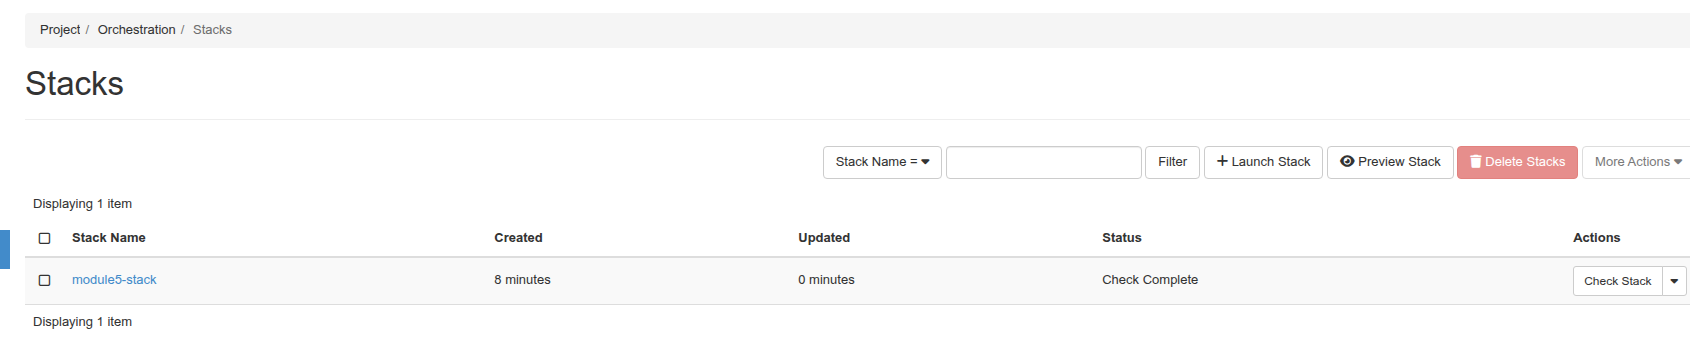
\includegraphics[width=0.88\linewidth]{img/m5-heat-stack-create-complete.png}
\caption{Heat stack \texttt{module5-stack} hoàn tất khởi tạo ở trạng thái thành công.}
\label{fig:m5_stack_status}
\end{figure}

\begin{figure}[H]
\centering
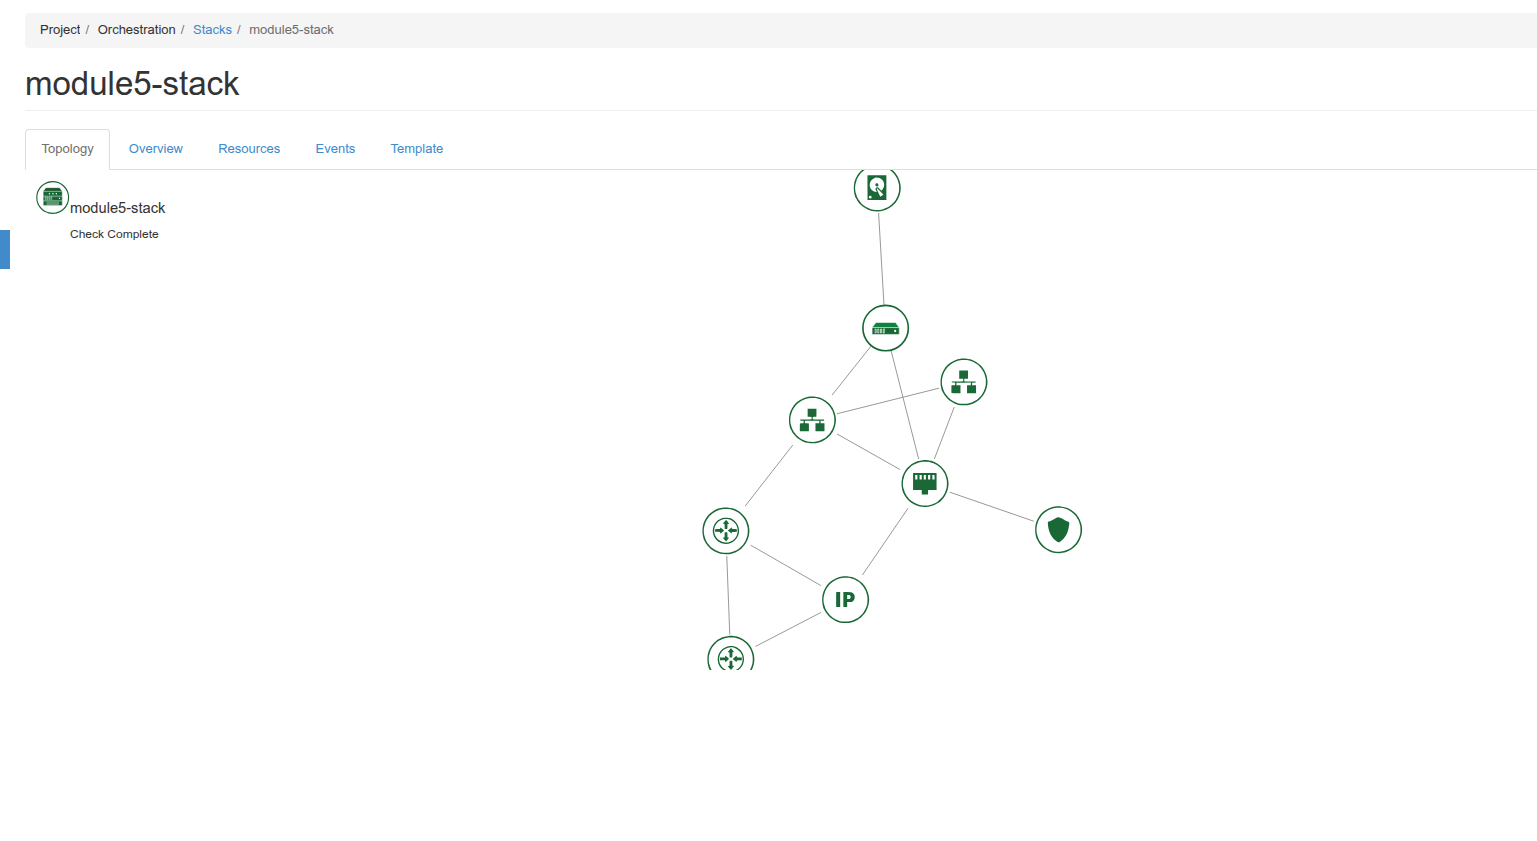
\includegraphics[width=0.88\linewidth]{img/m5-heat-stack-topology-graph.png}
\caption{Cây đồ thị phụ thuộc tài nguyên của Heat render trực quan trên Horizon.}
\label{fig:m5_stack_topology}
\end{figure}

Kết quả thực nghiệm cho thấy quy trình tự động hóa diễn ra chính xác và ổn định:
\begin{itemize}
    \item \textbf{Trạng thái Hoàn tất Cấp phát (Hình~\ref{fig:m5_stack_status}):} Heat Engine giải quyết thành công toàn bộ đồ thị phụ thuộc giữa các tài nguyên và chuyển stack sang trạng thái \texttt{CREATE\_COMPLETE} chỉ sau khoảng 60 giây.
    \item \textbf{Trực quan hóa Đồ thị Cấu trúc (Hình~\ref{fig:m5_stack_topology}):} Trên bảng điều khiển Horizon, cây topo tài nguyên hiển thị mạch lạc sự gắn kết giữa server, cổng mạng, nhóm bảo mật và volume lưu trữ theo đúng thiết kế khai báo.
    \item \textbf{Phân giải Tự động Đầu ra (Output Resolution):} Khối \texttt{outputs} của template tự động trả về đường dẫn URL công khai kèm địa chỉ Floating IP. Nhóm chúng em có thể truy cập ngay vào dịch vụ web qua trình duyệt mà không cần thêm bất kỳ thao tác cấu hình thủ công nào.
\end{itemize}

